\documentclass[border=10pt,tikz]{standalone}
\usepackage{tikz}
\usetikzlibrary{positioning,arrows.meta,shapes}
\begin{document}
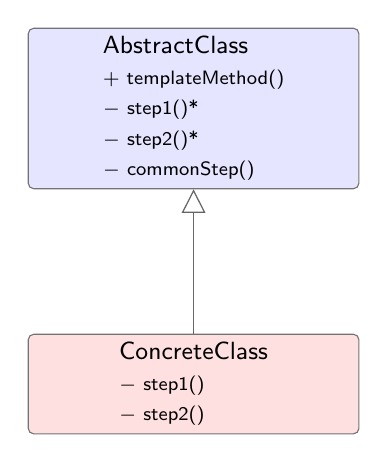
\begin{tikzpicture}[
  font=\sffamily\small,
  cls/.style={rectangle, rounded corners=2pt, draw=black!55, line width=0.4pt,
              minimum height=8mm, minimum width=42mm, inner sep=3pt, fill=white, align=left},
  abs/.style={cls, fill=blue!10},
  con/.style={cls, fill=red!12},
  inh/.style={-{Triangle[length=3mm,width=3mm,open]}, draw=black!60, line width=0.45pt}
]
\node[abs] (a) at (0, 1.5) {AbstractClass \\
  \scriptsize $+$ templateMethod() \\
  \scriptsize $-$ step1()* \\
  \scriptsize $-$ step2()* \\
  \scriptsize $-$ commonStep()};
\node[con] (c) at (0,-2)   {ConcreteClass \\
  \scriptsize $-$ step1() \\
  \scriptsize $-$ step2()};

\draw[inh] (c.north) -- (a.south);
\end{tikzpicture}
\end{document}
